\documentclass[11pt]{article}

\usepackage{amsmath,amssymb,amsthm,setspace,tabto,fancyhdr,sectsty,mathtools}
\usepackage{titleps}
\usepackage[left=1.00in,right=1.00in,top=0.75in,bottom=1.50in]{geometry}
\usepackage{graphicx}
\graphicspath{ {assets/note2/} }

% start pdfinlimg (GPLv3, https://github.com/zerotoc/pdfinlimg/blob/master/pdfinlimg.sty)
\newcommand{\pdfinlimg}[5]{
\makebox[#1cm][l]{\immediate\pdfliteral{
  q
  #3 0 0 #4 0 0 cm
  #1 0 0 #2 0 0 cm
  0.885 0 0 0.885 0 0 cm 
  BI
  /W #3
  /H #4
  /CS /RGB
  /BPC 8
  /F [ /AHx /Fl ]
  ID
  #5>
  EI
  Q
}\vbox to #2cm{}}
}
% end pdfinlimg

% BEGIN PARAGRAPH STUFF
\usepackage[utf8]{inputenc}
\usepackage[english]{babel}
 
\setlength{\parindent}{4em}
% \setlength{\parskip}{1em}
\renewcommand{\baselinestretch}{1}
% END PARAGRAPH STUFF

% useful commands
\DeclarePairedDelimiter{\ceil}{\lceil}{\rceil}
\DeclarePairedDelimiter{\floor}{\lfloor}{\rfloor}

\newpagestyle{footers} {
    \sethead{}{}{}
    \setfoot{\small Intro to Crypto and Blockchain, Note \notenum}{\thepage}{\small Lin, Akhtar}
    \footskip = 45pt
}

\fancypagestyle{firstpage} {
    \vspace*{3\baselineskip}
    \footskip = 0pt
    \renewcommand{\headrulewidth}{6pt}
    \chead{\rule{\textwidth}{6pt} \vspace{20pt}\\}
    \lhead{\setstretch{1.05}\Large\fontfamily{lmdh}\selectfont
    Introduction to Cryptocurrencies and Blockchain 
    \\ Lin, Akhtar}
    \rhead{\huge \fontfamily{lmdh}\selectfont    Note \notenum}
    \lfoot{\small Intro to Crypto and Blockchain, Note \notenum}
    \rfoot{\small Lin, Akhtar}
}
    
\sectionfont{\Large\fontfamily{lmdh}\selectfont}

% for initial paragraph indent
\usepackage{indentfirst}

% UPDATE THIS FOR EVERY NEW NOTE
\newcommand{\notenum}{2}

\pagestyle{footers}

\begin{document}
    \thispagestyle{firstpage}
    \vspace*{2\baselineskip}
    \section*{Bitcoin Protocol and Consensus: A High Level Overview}
    
    Beyond the excitement of Bitcoin, cryptocurrencies, and blockchain hides a confusion about what \textit{exactly} Bitcoin is and how it works at a technical level. This note is dedicated to explaining how Bitcoin works at a high level to build a mental model to prepare us for a more specific breakdown of Bitcoin's mechanics. 
    
    First, we will build Bitcoin from the ground up, explaining each of the system's key features and their necessity for Bitcoin to be distributed, decentralized, and trustless nature. Then, we will move on to discuss finer details in Bitcoin's implementation, such as a brief overview of mining and the anatomy of key data structures.
    
    \section*{Bitcoin from the Ground Up}
    
    To fully understand how Bitcoin works, we start by attempting to build Bitcoin from scratch. Each time a major flaw is detected, a new feature must be built in to resolve the problem. By the end of this section, we will have built Bitcoin from the ground up. Keep in mind that our goal is to create a currency that requires no central entity. Let us start off by considering two users of this currency, Alice and Bob.
    
    \textbf{First step:} Establishing a system that allows users to write and sign messages describing transactions, the primary value of currency. Each transaction would be broadcast to the world (more specifically, every other user of Bitcoin). Reasoning: If there exists no central third party to verify history, then \underline{every other member of the community} becomes the third party. For Alice to send Bob one bitcoin, she would announce to the world, ``I, Alice, am giving Bob one bitcoin," and the world would take note. A problem arises if Alice, intentionally or not, sends multiple identical messages to Bob. If she says five times in a row that she wants to give one bitcoin to Bob, did she accidentally repeat herself? Did she mean to send five bitcoins, or only one? The ability to send the same money multiple times would even give Alice the opportunity to spend more money than she has. 
    
    \textbf{Second step:} To prevent ambiguity, we introduce uniquely identifiable serial numbers for each transaction conducted on the system. If Alice were to send one bitcoin to Bob now, she would announce ``I, Alice, am giving Bob one bitcoin with serial number \#\#\#\#." Modern banks use similar serial numbers to keep track of their transactions. If our version of Bitcoin were to implement serial numbers, it must need a centralized bank to manage serial numbers, along with transactions and balances. However, this defeats the purpose of a decentralized currency and puts us right back where we started.
    
    \textbf{Third step:} Make everyone the bank. Have every user of Bitcoin store a complete record and serve as a witness and third party to all transactions. We will refer to this shared ledger as the ``blockchain." (We will elaborate on blockchains later.) In this new scheme, Alice may send Bob a transaction, and Bob will announce the transaction to the world. Other users update their records accordingly, and everyone keeps track of the amount of bitcoins each individual owns. What if, \newpage
    \noindent however, Alice double spends on Bob and Charlie? In other words, if Alice sends the same bitcoin to Bob and Charlie, how does the system know which transaction is valid, if any? Simply  rejecting the later transaction is unreliable, as in the real world of dropped packets (lost information) and unreliable connections, network speed varies too much. Some users may even see one transaction before the other.
    
    \textbf{Fourth step:} To address this problem, we ensure that the network confirms the validity of the transaction before allowing a recipient of funds to assume a successful transfer. edit the transaction sequence as follows: Alice sends a transaction to Bob, who then announces the transaction to the world. Everyone then verifies the transaction for Bob's protection. If Alice were to send the same funds to Charlie, those verifying would inform Bob and Charlie of Alice's deceit. This prevents Alice temporarily, but the possibility remains for Alice to double spend on Bob and Charlie given persistence. If she goes so far as to fabricate several fake online identities, she can then masquerade as several unbiased third parties while selfishly and maliciously verifying her own transaction, as both Bob and Charlie are unaware that all these other people are actually Alice and acting in Alice's best interests rather than the interests of the whole group. This attack pattern, of creating many fake identities to subvert a system, is well-known as a \textbf{Sybil attack}.
    
    \textbf{Fifth step:} To solve the Sybil attack vulnerability of double spending, the system can make it expensive to verify transactions. By requiring users to submit proof of having spent some resource to confirm a pending transaction, they will think twice before spending time, money, and energy on this verification process. Here, we shall implement a \textbf{proof-of-work} protocol. In a proof-of-work consensus system, when Alice wishes to make a transaction, she announces this to the entire network, as before. To correctly verify a pending transaction, an user must do three things. (Let us call this user ``David.") First, David must check his records to validate the transaction (i.e. to check if the bitcoins involved have not been spent before, if the person sending bitcoins is the owner/allowed to spend those bitcoins). Second, to prove his commitment to honesty, he must do some work---in Bitcoin's case, compute the solution to a difficult, arbitrarily and systematically chosen mathematical puzzle. Third, he must announce the validity of the transaction back to the network, along with the solution to the puzzle. Other users in the system would then verify the solution of the puzzle and the transaction before appending the transaction to their records.
    
    The most important step in this process is the second, in which David must solve the math puzzle. By requiring users to solve this math puzzle, which takes a great deal of computational power, we deter users from spawning endless identities and double spending, as they are now solely limited by the amount of computational power they have and are willing to spend. To further analyze how this solves double spending, consider the case after this fifth step when Alice attempts to double spend with multiple identities. We easily see the difficulty of identifying dishonest and malicious actors before they display malicious behavior. By requiring a mathematical puzzle to be solved, the system makes it costly for any user in the network to verify transactions. A good way to understand proof-of-work is to view it as a competition. Users on the network are constantly in competition to verify their blocks of transactions. Malicious actors such as Alice are in constant competition with other users to verify transactions. As long as the majority of computational power is owned by honest users, then bad actors such as Alice will have difficulty double spending.
    
    \textbf{Conclusion:} In building the system from the ground up, we have highlighted the major features of Bitcoin. In the beginning, signed messages that are announced to the entire network formed the basis of the entire system. After adding serial numbers, the system was able to uniquely identify transactions. By making everyone in the network the ``bank," we implemented a blockchain, allowing for a shared record of transactions. Having everyone in the network verify transactions provided a much-needed increase in security. Finally, proof-of-work deters malicious actors in the network from double-spending, actualizing a secure and trustless system. 
    
    \section*{Basic Concepts -- Identity in Bitcoin}
    
    As described earlier, one of the most fundamental concepts in Bitcoin is sending money between \textbf{pseudonymns}. In Bitcoin, a pseudonym refers to a user's Bitcoin \textbf{address}, otherwise known as the hash of their public key.
    
    Bitcoin also buids on some cryptographic primitives. Most notably, Bitcoin uses \textbf{ECDSA (Elliptic Curve Digital Signature Algorithm)} to produce cryptographically secure public and private key pair functionality similar to username and password schemes. Additionally, Bitcoin uses a \textbf{cryptographic hash function} called \textbf{SHA-256} in its proof-of-work scheme. Hash functions take in an input and \textbf{deterministically} create an output of fixed size. (While SHA-256 technically can't take in input of \textit{any} size, the limitations are beyond the scope of data used in Bitcoin: one must exceed $2^{64} - 1$ bits to exceed the valid input size, making the limit almost entirely theoretical.) \underline{Cryptographic} hash functions, specialized hash functions designed for security, are one-way: for a given output, it is very difficult to find its corresponding input, and a small change in the input data completely changes the output. These properties of SHA-256 are effective in maintaining security and consistency across the Bitcoin network, including the proof-of-work scheme and distribution of Bitcoin addresses.
    
    Another key concept in Bitcoin is that bitcoin is untouchable by anyone aside from the rightful owner, for two reasons: 1) Discovering the correct private key for a public key requires a quantum computer to expect a solution within your lifetime, and 2) Two randomly chosen private keys are \textit{incredibly} unlikely (still an understatement) to correspond to the same public key. There are $2^{160}$ possible addresses. To put this massive number into perspective, consider the following. There are roughly $2^{63}$ grains of sand on the Earth. Doubling the exponent, $2^{126}$ is actually only 0.0000000058\% of $2^{160}$. We only reach $2^{160}$ if we imagine that for each of the $2^{63}$ grains of sand on Earth, there is another Earth, each with its own set of grains of sand. The number of bitcoin addresses is so large that the possibility of colliding with someone else's bitcoin whenever a user generates a public/private key pair is negligible. (For those curious, $2^{160}$ is exactly 1,461,501,637,330,902,918,203,684,832,716,283,019,655,932,542,976 -- \textit{Rustie}) 
    
    \section*{Transactions -- A Basic Version}
    
    Transactions are usually conducted through wallet software, although it is possible to do this manually. Wallet software automatically generates Bitcoin addresses for its users. Users can then receive money by sharing their addresses, or send money specifying an address and amount. In many online wallets, transactions can even be conducted easily via a series of QR codes (e.g. in the Coinbase interface.) Whenever a transaction is made, it is broadcast to the entire Bitcoin network, where the network verifies the transaction and adds it to the transaction history.
    
    \section*{Introduction to Transactions}
    
    When a user spends bitcoins, they are always spending bitcoins received in previous transactions. Transactions are mappings from inputs to outputs, where inputs and outputs each contain an address and an amount. For example, let's say Bob spends 0.05 BTC at a coffee shop. If the transaction input was 1.00 BTC, then the outputs would be 0.05 BTC to the coffee shop, and 0.95 BTC back to Bob. The reason for two outputs is because as per the Bitcoin system specification, inputs can only be spent once, creating the need for a change output (the 0.95 BTC) back to the sender. The Bitcoin network also imposes transaction fees: users are expected to construct transactions such that the input amount exceeds the output amount, and their difference equals the transaction fees collected by the network. In the previous example, if Bob sends 0.05 BTC to the coffee shop and only 0.94 BTC back to himself, then the difference in inputs and outputs (1.00 BTC - 0.05 BTC - 0.94 BTC = 0.01 BTC) equals the transaction fee. Keep in mind that transactions with lower transaction fees offered up to the network are less likely to get confirmed---if ever! (You will soon see that ``the network" is an abstraction referring to miners, which we will talk about later in this note.)
    
    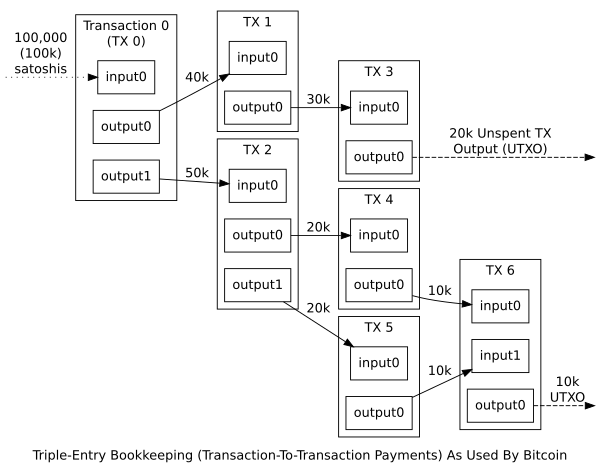
\includegraphics[scale=0.9]{transactions}
    
    \section*{Blocks and Blockchain}
    
    A \textbf{block} serves the purpose of containing an ordered bunch of transactions. Key characteristics of a block include time-stamps and (with the exception of the genesis block) references to the most recent previous block. Changing a transaction, the block's time-stamp, or the block's reference invalidates a block. This property ensures that blocks are immutable. A \textbf{blockchain}, as the word implies, is a series of blocks that are ``chained" together. Later parts of this note will discuss further a block's components.
       
   \section*{Basic Concepts -- UTXO Analogy}
   
    In Bitcoin, users do not have accounts from which they add or subtract value to determine the amout of bitcoin they own. Instead, users spend from unspent transaction outputs, or \textbf{UTXOs}. UTXOs can be thought of as the global set of unspent bitcoins. Instead of ``spending A bitcoin," it is more useful to think of a user as ``spending THIS bitcoin," as bitcoins are uniquely identified by their transaction outputs. (Think back to our reasoning for serialized currency in ``Bitcoin from the Ground Up.")
    
    Bitcoin is analogous to the Rai Stones of the Yap Islands. Rai Stones are large circular stone disks carved out of limestone by the Yapese, a Micronesian people, and used as currency. These Rai Stones were upwards of 3.6 meters in diameter and 4 metric tons heavy, too much for locals to move around regularly. Instead, to conduct transactions and exchange them for goods, the Yapese agreed on a system that revolved on trust and changing ownership of the Rai Stones. In a transaction, both parties would announce to the rest of the island that the transfer of ownership over stones was taking place. This is how Bitcoin works, as ownership of specific bitcoins are transferred between users during transactions. (There is a slight difference because bitcoins can be divided and renamed, but the concept remains true.)
    
    \begin{center}
    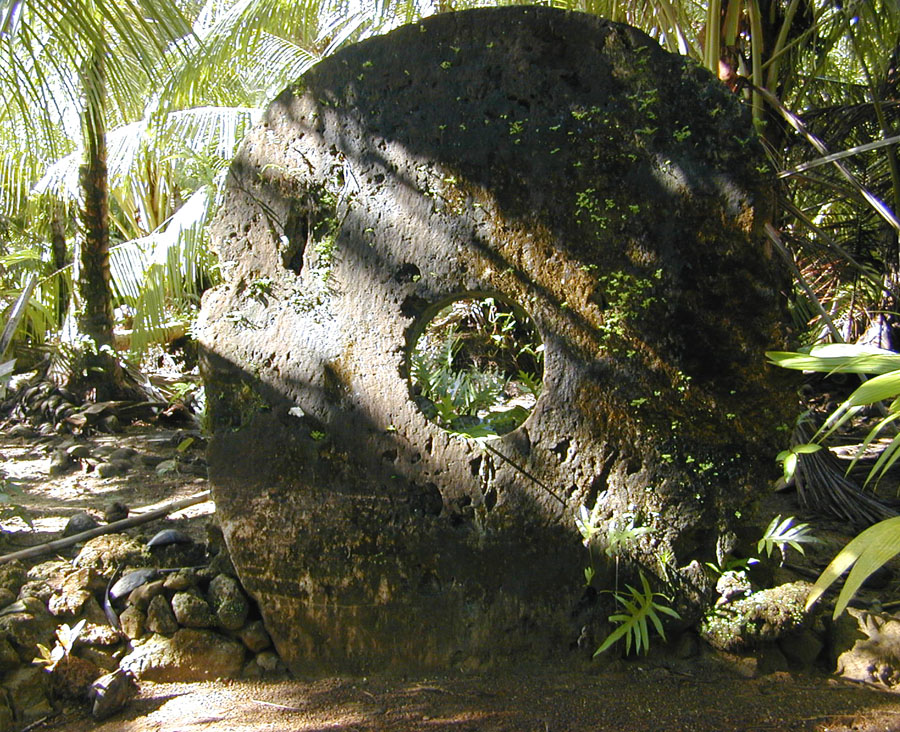
\includegraphics[scale=0.7]{rai}
    \end{center}
    
    \section*{Mining Sketch}
    
    Before exploring mining, we must first understand proof-of-work. Proof-of-work solves the double spending problem and is a \textbf{Byzantine consensus algorithm}, an algorithm which tolerates failures involving both faulty and malicious nodes. The former will behave in aimlessly incorrect ways, such as by sending repeat or corrupt messages. The latter intends to subvert the system, either by propagating false information or by preventing the system from coming to consensus. Proof-of-work is but one of many consensus algorithms, however, so keep in mind that it is not the be-all and end-all to decentralized consensus. Private and hybrid/consortium blockchains use alternative consensus algorithms, but because they are not public (and, by implication, not anonymized), the system depends on trusting a good majority of approved entities, opening up opportunities to use multitudes of various other consensus algorithms given certain assumptions of trust.
    
    In Bitcoin, \textbf{mining} serves various essential functions that uphold the entire Bitcion system. Primarily, it serves as a minting mechanism, ensuring fair distributions of coins via the proof-of-work challenge. (Some could argue against this, considering the presence of mining pools. More on this in a later note.) Additionally, the treasured block reward incentivizes \textbf{miners} to support the greater goal of securing the network. Countless miners maintaining network health and protecting distributed consensus ultimately determine Bitcoin's security and viability.
    
    \section*{Mining Sketch -- Finding Blocks}
    
    Every miner includes a special transaction called a \textbf{coinbase transaction} in a block's list of transactions. This transaction allows miners to receive a mining reward \big(currently at 12.5 BTC (6/20/17)\big) if they find a valid proof-of-work before every other miner. Miners who have found a valid proof-of-work have, in Bitcoin vernacular, ``found the block." The miner saves the block to his own blockchain, then broadcasts the block to the rest of the Bitcoin network. Other miners in the network would verify the block and then add it to their own copy of the blockchain.
    
    On average, a block is found every 10 minutes. Not by chance, but by design: because the average level of computational power (which we shall also refer to as ``\textbf{hash rate}") within the network constantly varies, the difficulty of the problem which miners solve (the proof-of-work puzzle) must adjust accordingly. Consider a scenario in which the difficulty remained constant: if the hash rate rises significantly (the expected long-term trend), then the puzzle becomes too easy to solve, and the proof-of-work no longer requires any work; and if the hash rate decreases significantly, then the network gets backed up because valid blocks are too difficult and time-consuming to generate. Hence, the puzzle's difficulty must adapt to remain relatively as difficult as before with the network's hash rate fluctuations. (We shall discuss further in Note 5, ``Mining.") 
    
    The block reward halves every 4 years; at the time of writing, the nearest instance of the block reward halving will be on July 9th, 2017. A halving block reward implies that bitcoins are in limited supply, i.e. deflationary, as the block reward will approach 0 over time and no more bitcoins will be minted. Around Year 2140, the maximum of 21 million bitcoins will be in circulation. There are approximately 15.2 million bitcoins in circulation today (6/19/17).
    
    Briefly, the process of mining can be described as follows: A miner attempts to generate a ``valid" block header. Before we discuss the definition of ``valid," let us look at what defines a potential block header:
    $$\mathit{Output} = \text{SHA-256}\big(\mathit{Merkle~Root} + \text{SHA-256}(\mathit{Previous~Block}) + \mathit{Nonce}\big) = \mathit{Block~Header}$$
    
    The output of the hash of three components, 1) the \textbf{Merkle root}, 2) a hash of a previous block header, and 3) a \textbf{nonce}, generates a block header. A Merkle root preserves a summary of transactions by using some useful cryptographic properties which we will discuss later. A nonce is an arbitrary number, the piece of the math puzzle miners search for, the coveted proof-of-work, and the only part of this equation that changes. A miner uses SHA-256 to hash together the Merkle root, a nonce, and a hash of the previous block. 
    
    A ``valid" block header must contain a prerequisite number of leading zeroes agreed upon by the network per the ``difficulty." The higher the difficulty, the more leading zeroes required for a valid block header, and vice versa. Validity is defined as leading zeroes because a) any arbitrary pattern could have been selected (leading number of sixes, sequential order of digits), but leading zeroes happened to be selected, and b) the required amount of leading zeroes is easy to adjust, fulfilling our desire from before for an adjustable difficulty. The solution (proof-of-work) that miners vie for is defined as an output that generates a valid block header. The difficulty of the puzzle is constantly adjusted every 2016 blocks (every two weeks at 10 minutes/block).
    
   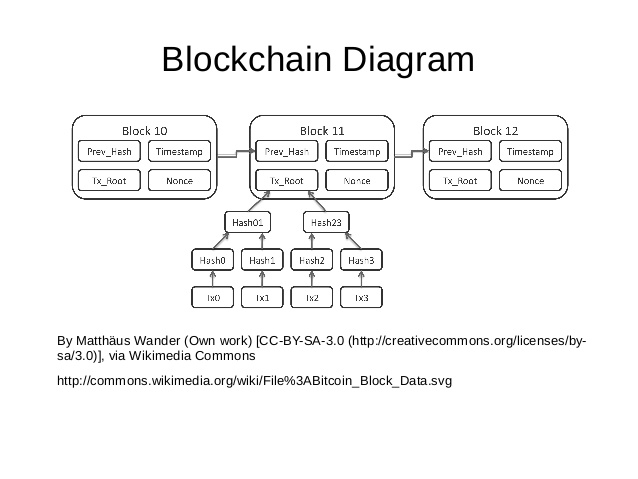
\includegraphics[scale=0.65]{blockchain_diagram}
   
   \section*{Transaction Flow}
   
   \textit{To more clearly illustrate the process of making a transaction, consider the following example:}
   
   Imagine Alice wants to send money to Bob. Alice would first sign a transaction and broadcast this to the network. Miners would then receive and verify the transaction by checking for a) a valid signature and b) sufficient funds. When a miner finds the proof-of-work, thereby solving the block, they would then broadcast the block to the network. As the block propagates, other miners would verify the block themselves. At any given point in time, the longest blockchain is assumed to be the most valid, and since miners are constantly competing for the block reward, they immediately start work on the next block's problem.
   
   Keep in mind that almost all blocks contain hundreds of transactions, so as to increase a miner's transaction fees per block, and that miners prioritize transactions offering the highest fees.
   
   \section*{51\% Attacks}
   
   Bitcoin assumes that a majority of the network is honest. By implication, an honest majority will form the longest proof-of-work chain because the majority of the network's hash rate (owned by the honest) would create blocks faster than malicious entities would. Since miners have no incentive to work on a short, malicious chain that will not be recognized as truth in the future, thus offering no block reward or longevity of transactions, miners will work on the longest chain. However, this assumption puts Bitcoin at risk of a \textbf{51\% attack}, an attempt to overwhelm the honest mining power of a network. While it is possible, amassing 51\% of the network's hash power is highly unlikely. (We will also discuss this further in ``Game Theory.")
   
   \section*{Forking and Consensus Updates}
   
   With time, Bitcoin's protocol and software must update to remain efficient and secure. However, nodes may choose to opt out of updating their protocol, causing a split known as a \textbf{fork}. There are two categories of forks, each with drastically different implications.
   
   In a \textbf{hard fork}, the new version of the consensus protocols is incompatible with the previous because of loosened requirements upon blocks. In other words, hard forks are not forwards compatible. A hard fork causes a permanent divergence in the blockchain. Nodes running an old version of the Bitcoin software would see the new transactions as invalid and thus hard forks are not backwards compatible. An issue can arise when upgraded nodes mine on the new forked blockchain, and non-upgraded nodes continue mining on the old chain. With enough community support, both chains could survive, and we can see this in Ethereum and Ethereum Classic.
   
   \smallskip
   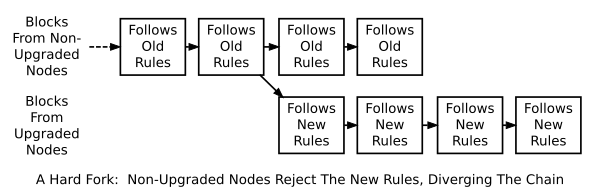
\includegraphics[scale=0.9]{hard_fork}
   \smallskip
   
   A \textbf{soft fork} tightens the protocol, meaning that old nodes will always accept blocks from new nodes, and the new chain remains valid under old consensus rules. Changes brought about by soft forks are forwards compatible but not backwards compatible, as only a subset of previously types of blocks are acceptable. Although non-upgraded nodes will still be able to see new transactions as valid, they will not be able to mine, as upgraded nodes will reject their blocks. If a majority of the network adopts the new protocol of the soft fork, the network ultimately upgrades to the newer consensus rules.
   
   \medskip   
   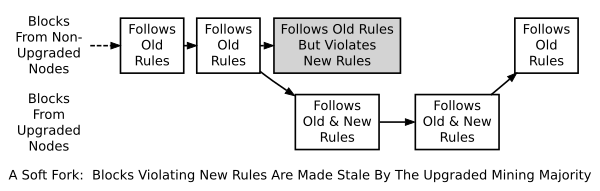
\includegraphics[scale=0.9]{soft_fork}
  
   \section*{Merkle Trees}
  
%   \textbf{Merkle trees}: fundamental datastructures granting immutability to Bitcoin transactions. 
   
   \medskip
   \begin{center}
   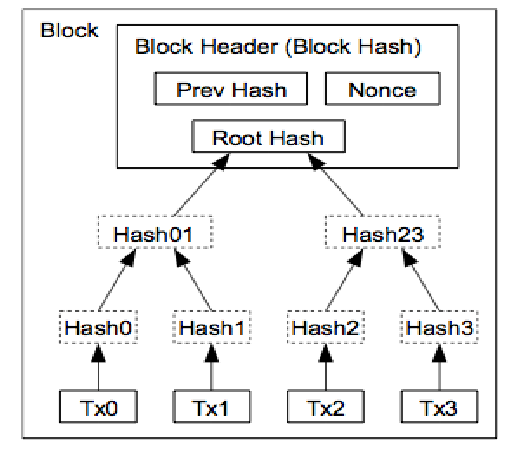
\includegraphics[scale=0.6]{merkle}
   \end{center}
   \smallskip
   
   As seen in the diagram, a \textbf{Merkle tree} is a fundamental data structure, ``gluing" transactions together and immensely facilitating error detection. It is a \textbf{binary tree} in which every non-leaf node equals the hash of the values of its child nodes. To construct a Merkle tree, a miner begins by lining up all transactions, hashing them all once, then hashing them up in pairs up to the final hash. In this diagram, ``Tx\#" generates ``Hash\#" in the first hashing step. On the right, hashing ``Hash2" and ``Hash3" together yields ``Hash23," and same on the left. When all transactions are hashed together, the resulting structure is the \textbf{Merkle root}, which is then stored in the block. The rest of the Merkle tree is then discarded to save space in the block.
   
   Let's finally understand part of the blockchain's immutability: imagine that a malicious user tampered with a transaction. (Remember, even a minuscule change in a hash function's input drastically changes the output.) With the change of that transaction follows a change in that transaction's hash value within the Merkle tree, bubbling up to the Merkle root. Due to the properties of SHA-256 and the number of times hashing is required in the process of constructing a Merkle tree, the block containing the corrupted transaction has a drastically different block header than before. The hash of the nonce, Merkle root hash, and previous block hash would then not remain valid per our prior definition, invalidating the block and informing the network of attempted fraud.
   
    
    
    % BEGIN KEY TERMS
    \newpage
    \thispagestyle{firstpage}
    \vspace*{2\baselineskip}
    \section*{Key Terms}
    \noindent A collection of terms mentioned in the note which may or may not have been described. Look to external sources for deeper understanding of any non-crypto/blockchain terms.
    \begin{enumerate}
        \item \textbf{Address} --- In the context of Bitcoin (and other pseudonymous/public blockchains), an arbitrary number representing a user's identity. Others can send money to this address, and a user can send money from this address.
        \item \textbf{Binary tree} ---
        \item \textbf{Block} --- 
        \item \textbf{Blockchain} --- 
        \item \textbf{Byzantine consensus algorithm} --- 
        \item \textbf{Coinbase transaction} --- 
        \item \textbf{Cryptographic hash function} --- 
        \item \textbf{Deterministic} --- 
        \item \textbf{ECDSA} --- Short for \underline{E}lliptic \underline{C}urve \underline{D}igital \underline{S}ignature \underline{A}lgorithm. In Bitcoin, ECDSA is used to generate public and private key pairs, which in turn allows users to sign transactions such that third parties can verify the authenticity of the signature while retaining exclusive ability to create the signature.
        \item \textbf{Fork} --- 
        \item \textbf{Hard fork} --- 
        \item \textbf{Hash rate} --- 
        \item \textbf{Merkle root} --- 
        \item \textbf{Merkle tree} --- 
        \item \textbf{Proof-of-work} --- A piece of data which is costly to produce but easy for others to verify and which satisfies certain requirements.
        \item \textbf{Nonce} --- 
        \item \textbf{Pseudonym} --- A false name. (In Bitcoin context, see: \textit{Address})
        \item \textbf{SHA-256} --- A cryptographic hash function used in various parts of the Bitcoin network such as the proof-of-work challenge.
        \item \textbf{Soft fork} --- 
        \item \textbf{Sybil attack} --- A strategy by which a single entity generates additional identities, often a great many, in order to gain substantial undue influence in a peer-to-peer network. The rest of the network is not aware that all these identities belong to one person in a successful attack.
        \item \textbf{51\% attack} --- 
    \end{enumerate}
    % END KEY TERMS
\end{document}